% 100
\begin{textarea}[]
	\only<1>{
		\begin{columns}[c] 
			\column{.5\textwidth} 
			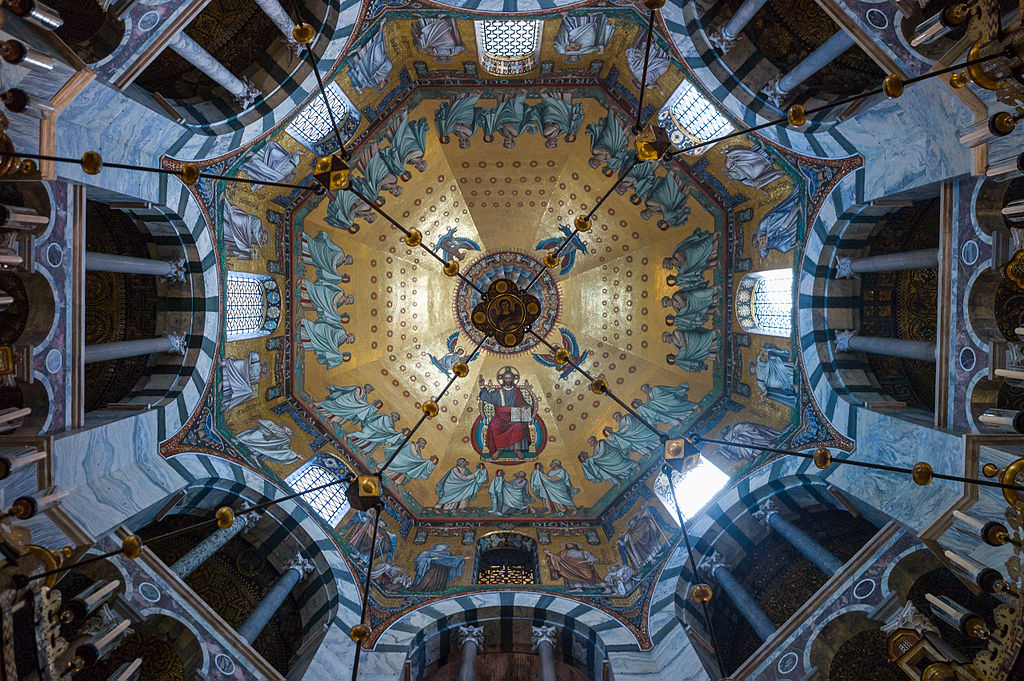
\includegraphics[height=0.6\linewidth]{categories/media/Aachener_Dom_August_2014}
			\column{.5\textwidth}
			What a nice ceiling this building has...  				
		\end{columns}
	}
	\only<2>{
		What is Aachen cathedral?
	}
\end{textarea}

% 200
\begin{textarea}[]
	\only<1>{
		\begin{columns}[c] 
			\column{.5\textwidth} 
			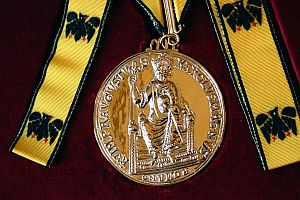
\includegraphics[height=0.5\linewidth]{categories/media/CharlemagnePrize}
			\column{.5\textwidth}
			Parts of this building date back to Charlemagne,
			whose price is rewarded here once a year.
		\end{columns}
	}
	\only<2>{
		What is Aachen City Hall?
	}
\end{textarea}




% 300
\begin{textarea}[]
  \only<1>{
    \begin{columns}[c] 
      \column{.5\textwidth} 
      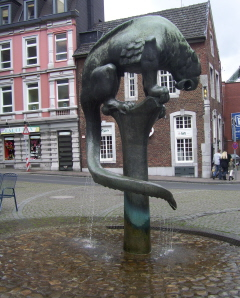
\includegraphics[height=1.0\linewidth]{categories/media/Brunnen-am-buechel}
      \column{.5\textwidth}
      Drunk husbands used this guy as an excuse to come home late.
    \end{columns}
  }
  \only<2>{
    What is the Bahkauv?
  }
\end{textarea}

% 400
\begin{textarea}[]
	\only<1>{
		\begin{columns}[c] 
			\column{.5\textwidth} 
			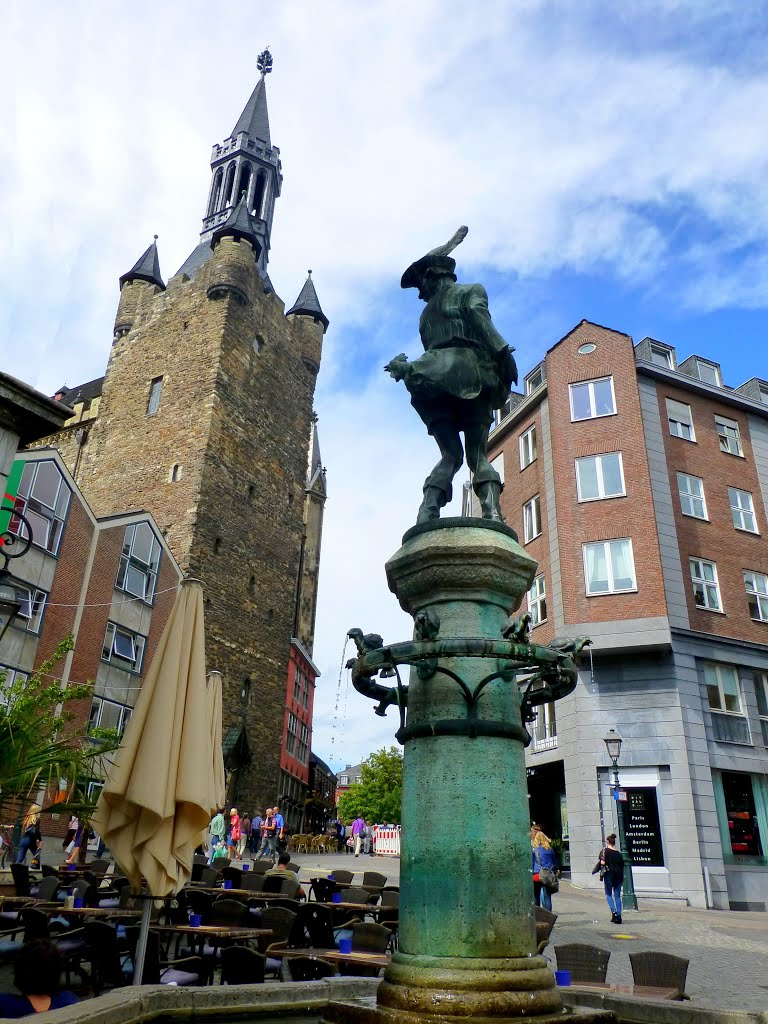
\includegraphics[height=1.0\linewidth]{categories/media/huehnerdieb}
			\column{.5\textwidth}
			You probably don't want to see this guy on the market, especially not if you sell chicken.    
		\end{columns}
	}
	\only<2>{
		What is the H\"uhnerdieb?
	}
\end{textarea}


% 500
\begin{textarea}[]
	\only<1>{
		\begin{columns}[c] 
			\column{.5\textwidth} 
			\includegraphics[height=1.0\linewidth]{categories/media/Löwenstein_House_Aachen}
			\column{.5\textwidth}
			It is one of Aachen's oldest buildings and can be found on the market square.
		\end{columns}
		
	}
	\only<2>{
		What is L\"owenstein house?
	}
\end{textarea}





% % % % % % % % % % %
\begin{textarea}[]
	\only<1>{
		\centering
		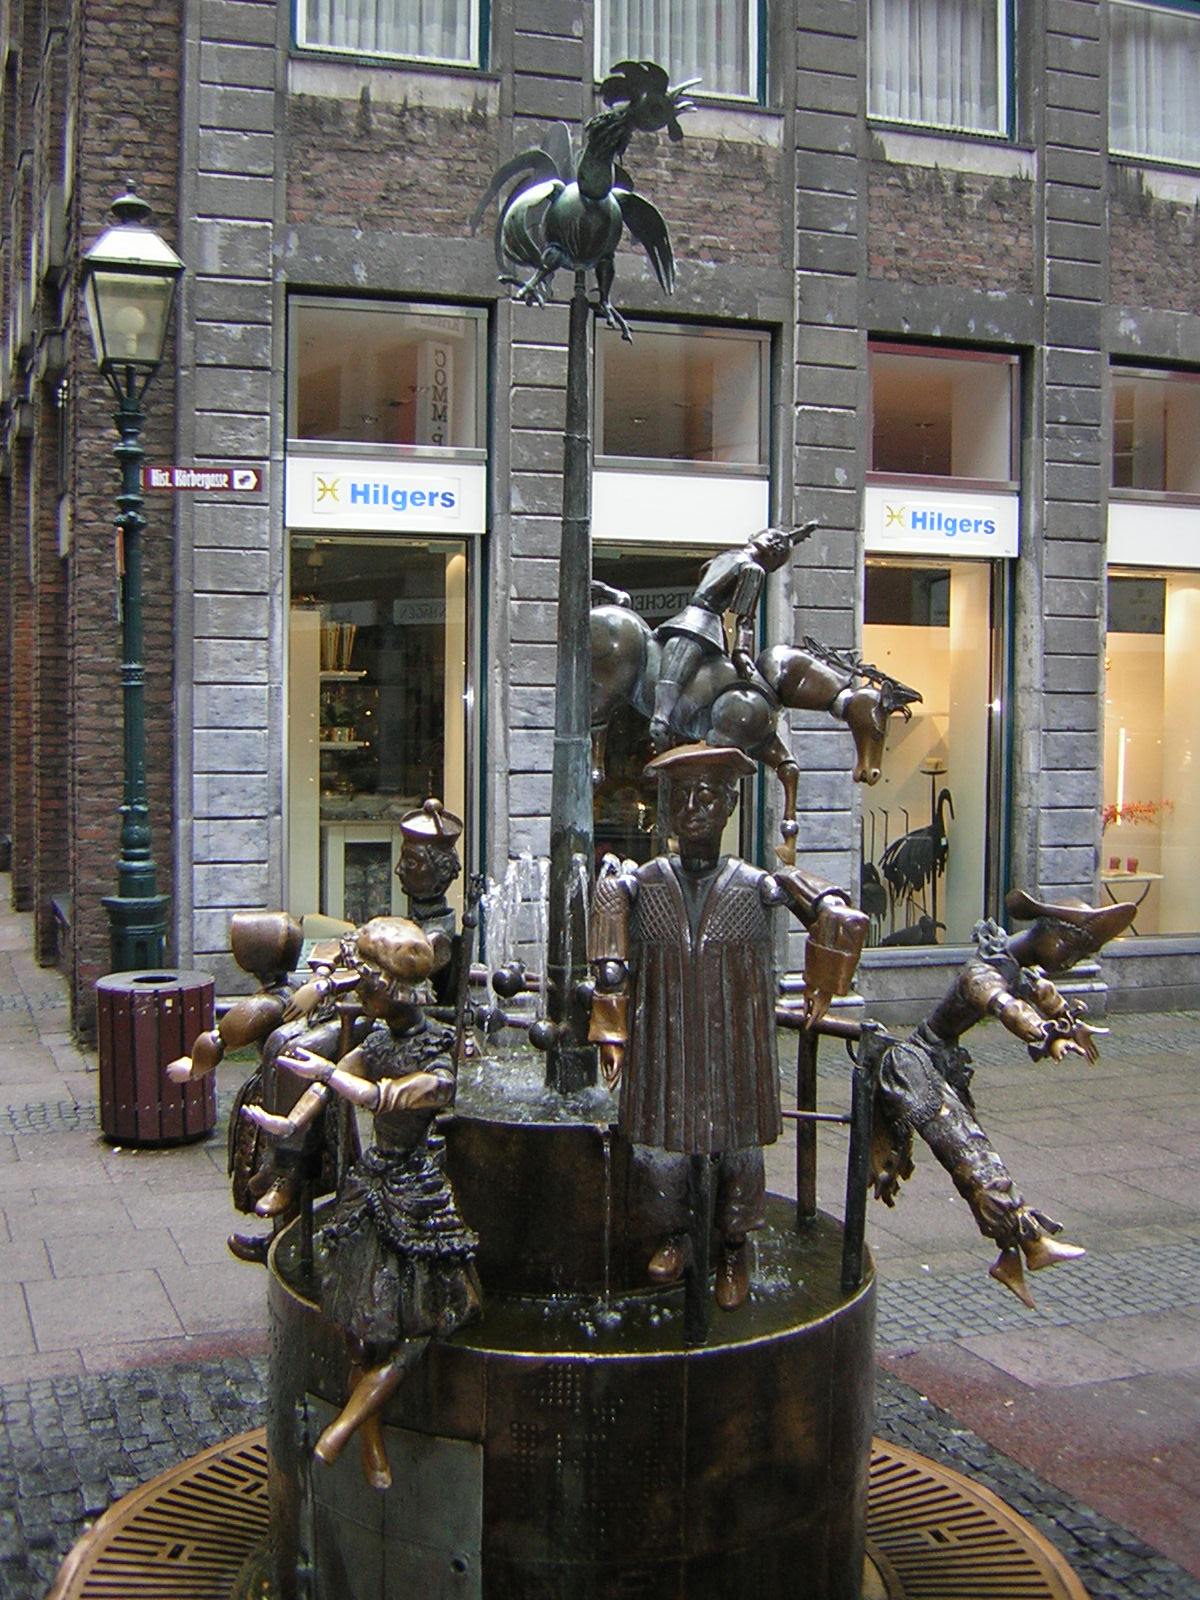
\includegraphics[height=0.5\linewidth]{categories/media/Puppenbrunnen_in_Aachen.JPG}
	}
	\only<2>{
		What is the Puppenbrunnen?
	}
\end{textarea}

\begin{textarea}[]
	\only<1>{
		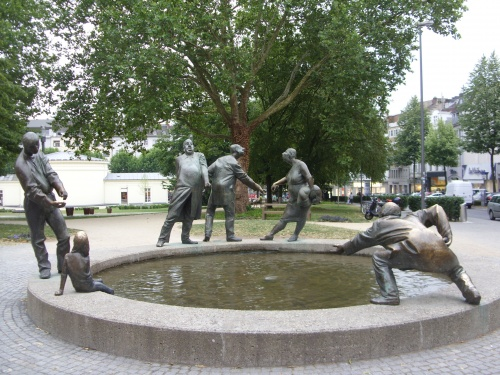
\includegraphics[height=0.5\linewidth]{categories/media/LaufDesGeldes}
	}
	\only<2>{
		What is Kreislauf des Geldes?
	}
\end{textarea}